Das OctoPrint-Webinterface ist das Kontrollinterface des Druckers. Sofern man mit dem gleichen Netzwerk verbunden ist, sollte es über "`octopi.local"', bzw. der IP des RaspberryPi, im Browser-Fenster erreichbar sein. Mit ihm lassen sich Drucke starten und stoppen, sowie deren Fortschritt überwachen etc.

\subsubsection{Starten eines Druckes}
Um über das Webinterface einen Druck an zu fangen, gibt es zwei Möglichkeiten:
\begin{itemize}[noitemsep]
\item Hochladen eines 3D-Modells auf das Webinterface
\item Nutzung eines externen Slicers - z.B. Slic3r (nur für erfahrene Nutzer!)
\end{itemize}
Dieses Handbuch wird sich lediglich mit dem Webinterface des Druckers beschäftigen. Zur Nutzung und Konfiguration eines externen Slicers sollten dessen Bedienungshinweise beachtet werden. Ebenfalls wird erwartet, dass bereits ein korrekt orientiertes und druckbares Modell vor liegt - hierfür siehe Kapitel \ref{ch:DesignChoices}, Seite \pageref{ch:DesignChoices}.

Zum Starten des Druckes eines 3D-Modells muss folgendes getan werden:

\paragraph{Erstellung des 3D-Modells:} Es muss ein fertiges, als STL formatiertes Modell vor liegen, welches an den Drucker angepasst wurde. Hierfür muss gegebenenfalls aus dem Design-Programm exportiert werden (z.B. FreeCAD), oder das Modell gerendert werden (z.B. OpenSCAD). Es sollte auch darauf geachtet werden, dass das Modell in der richtigen Orientierung ist (flache Seite unten), sowie für den Drucker geeignet designt wurde.

\paragraph{Vorbereitung des Druckers:} Um den Druck korrekt zu starten, muss der Drucker bereit dafür sein. Hierfür muss dieser an und im "`Ruhezustand"' sein, d.h. er darf nicht momentan am Drucken sein, und es darf sich kein Plastik auf dem Druckbett befinden. Ist dies jedoch der Fall, so muss das Druckbett gereinigt werden, bis alle Hindernisse aus dem Weg sind. \emph{Ein Druck darf nur gestartet werden wenn sicher gestellt wird dass das Druckbett frei ist!}

\paragraph{Hochladen:} Das 3D-Modell kann nun auf den OctoPrint-Server geladen werden. Hierfür kann man es entweder via Drag \& Drop auf das Webinterface ziehen, oder auf den "`Upload"'-Knopf in der unteren linken Seite (unter dem Datei-Dialog) drücken, und es im darauf folgenden Dialogfenster aus wählen.

\paragraph{Slicen:} Das Slicen des Modells, also die Zerlegung in für den Drucker verständlichen Code, wird direkt vom RaspberryPi übernommen. Jedoch muss vorher noch vom Nutzer einiges ausgewählt werden:\\
\begin{center}
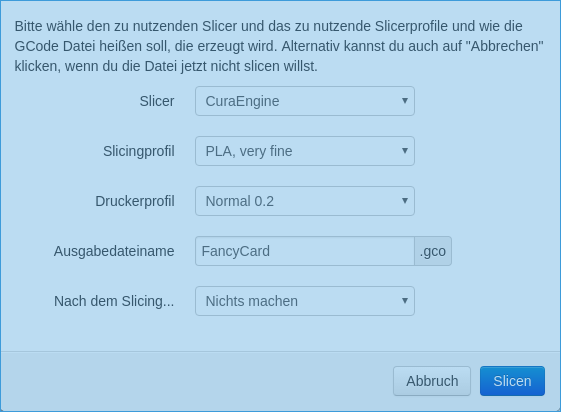
\includegraphics[width=0.9\textwidth]{Bilder/OPSliceWindow.png}
\end{center}
In diesem Fenster müssen nun folgende Parameter angepasst werden:
\begin{itemize}[noitemsep]
\item Das Slicingprofil muss korrekt ausgewählt werden, d.h. es muss das richtige Material (meist PLA!), sowie die gewünschte Qualität ausgewählt werden.
\item Das Druckerprofil muss auf "`Normal 0.3"' gesetzt werden, sofern dies nicht der Fall ist!
\item "`Nach dem Slicing"' sollte auf "`Drucken"' gesetzt werden.
\end{itemize}
Nun kann auf "`OK"' gedrückt werden. Das Modell sollte nun vom RaspberryPi verarbeitet werden, und der Druck sollte starten.


\paragraph{Druckstart:} Nachdem nun das Modell geladen und vorbereitet wurde, wird der Drucker sofort mit dem Druck an fangen. Hierfür ist es sehr wichtig zumindest die erste Schicht gut im Auge zu behalten! Oftmals schlägt ein Druck wegen eben jener ersten Schicht fehl, es ist dementsprechend unabdingbar dass dafür gesorgt wird dass diese gut sitzt! Sollte der Druck hier fehl schlagen, so muss Abgebrochen und neu gestartet werden (siehe \textbf{LINK EINFÜGEN}). 

Auch ist während des Druckens selbst regelmäßig ein Auge auf den Prozess zu halten - es kann jederzeit einen Fehler geben, der den Druck fehl schlagen lässt oder ernsthafte Probleme verursachen kann, \emph{ohne dass die Maschine dies bemerken kann.} Empfehlenswert ist eine Überprüfung des Druckes alle 15 bis 30 Minuten; dies kann über den "`Steuerung"'-Tab im OctoPrint Fenster erledigt werden, welcher einen Webcam-Livestream an zeigt.